Anacleta, ciclista apasionada,
planifica su próxima ruta
usando mapas que descargó de internet.
Cada mapa es un diccionario
que asocia a cada ciudad
el conjunto de sus ciudades vecinas.
Dos ciudades son vecinas
cuando hay un camino directo que las une.

Por ejemplo,
la siguiente figura muestra un mapa con siete ciudades,
junto con el diccionario que le corresponde:

\begin{minipage}[T]{.45\textwidth}
  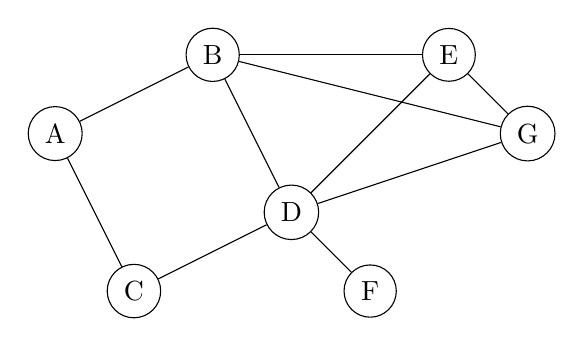
\begin{tikzpicture}[scale=1]
    \node[draw, circle] (A) at (0, 2) {A};
    \node[draw, circle] (B) at (2, 3) {B};
    \node[draw, circle] (C) at (1, 0) {C};
    \node[draw, circle] (D) at (3, 1) {D};
    \node[draw, circle] (E) at (5, 3) {E};
    \node[draw, circle] (F) at (4, 0) {F};
    \node[draw, circle] (G) at (6, 2) {G};
    \draw (A) -- (B);
    \draw (A) -- (C);
    \draw (B) -- (D);
    \draw (B) -- (E);
    \draw (B) -- (G);
    \draw (C) -- (D);
    \draw (D) -- (E);
    \draw (D) -- (F);
    \draw (D) -- (G);
    \draw (E) -- (G);
  \end{tikzpicture}
\end{minipage}
\hfil
\begin{minipage}[T]{.45\textwidth}
  \lstinputlisting[linerange=EJEMPLO-FIN\ EJEMPLO]{mapas/solucion.py}
\end{minipage}

Anacleta desea planificar una ruta
(es decir, una secuencia de ciudades para visitar)
y ver si es posible hacerla en mismo orden que a ella le interesa.
No obstante,
ella no se siente capacitada para hacer trayectos muy largos,
por lo que en un día sólo le interesa ir de una ciudad a otra vecina.
Sólo cuando se sienta especialmente vigorosa
intentará seguir de largo para llegar a una próxima ciudad.

\begin{enumerate}[leftmargin=0pt,label=\emph{\alph*})]

  \item
    Escriba la función \li!son_vecinas(mapa, p, q)!
    que retorne un valor booleano
    indicando si las ciudades \li!p! y \li!q!
    son o no vecinas en el \li!mapa!
    (es decir, si se puede ir directamente de \li!p! a \li!q!
    sin pasar a través de ninguna otra ciudad).
    \lstinputlisting[linerange=CASO\ 1-FIN\ CASO\ 1]{mapas/solucion.py}

  \item
    Escriba la función \li!tienen_vecino_en_comun(mapa, p, q)!
    que retorne un valor booleano
    indicando si las ciudades \li!p! y \li!q!
    tienen o no un vecino en común en el \li!mapa!
    (es decir, si se puede ir de \li!p! a \li!q!
    pasando a través de una sola otra ciudad).
    \lstinputlisting[linerange=CASO\ 2-FIN\ CASO\ 2]{mapas/solucion.py}

  \item
    Escriba la función \li!existe_ruta(mapa, ruta)!
    que retorne un valor booleano
    indicando si es posible hacer la \li!ruta! en el orden indicado.
    El parámetro \li!ruta! es una lista de ciudades.
    \lstinputlisting[linerange=CASO\ 3-FIN\ CASO\ 3]{mapas/solucion.py}

\end{enumerate}

Conteste al reverso de esta misma hoja.

